\let\negmedspace\undefined
\let\negthickspace\undefined
\documentclass[journal,12pt,onecolumn]{IEEEtran}
\usepackage{cite}
\usepackage{amsmath,amssymb,amsfonts,amsthm}
\usepackage{algorithmic}
\usepackage{graphicx}
\usepackage{textcomp}
\usepackage{xcolor}
\usepackage{txfonts}
\usepackage{listings}
\usepackage{enumitem}
\usepackage{mathtools}
\usepackage{gensymb}
\usepackage{comment}
\usepackage{caption}
\usepackage[breaklinks=true]{hyperref}
\usepackage{tkz-euclide} 
\usepackage{listings}
\usepackage{gvv}                                        
%\def\inputGnumericTable{}                                 
\usepackage[latin1]{inputenc}     
\usepackage{xparse}
\usepackage{color}                                            
\usepackage{array}                                            
\usepackage{longtable}                                       
\usepackage{calc}                                             
\usepackage{multirow}
\usepackage{multicol}
\usepackage{hhline}                                           
\usepackage{ifthen}                                           
\usepackage{lscape}
\usepackage{tabularx}
\usepackage{array}
\usepackage{float}
%\newtheorem{theorem}{Theorem}[section]
%\newtheorem{theorem}{Theorem}[section]
%\newtheorem{problem}{Problem}
%\newtheorem{proposition}{Proposition}[section]
%\newtheorem{lemma}{Lemma}[section]
%\newtheorem{corollary}[theorem]{Corollary}
%\newtheorem{example}{Example}[section]
%\newtheorem{definition}[problem]{Definition}

\begin{document}

\title{1.8.11}
\author{AI25BTECH11035 - SUJAL RAJANI}
% \maketitle
% \newpage
% \bigskip
%\begin{document}
{\let\newpage\relax\maketitle}
%\renewcommand{\thefigure}{\theenumi}
%\renewcommand{\thetable}{\theenumi}
% \newpage
% \bigskip
\textbf{Question}:
\\
\noindent AOBC is a rectangle whose three vertices are vertices $\vec{A}(0,3),\vec{O}(0,0),\vec{B}(5,0)$. The 
length of diagonal is \underline{\hspace{2cm}}.
\textbf{Solution:} 
\\
From the given information,
\begin{align}
			\vec A = \myvec{0\\3},\vec O = \myvec{0\\0},\vec{B} = \myvec{5\\0} 
\end{align}
Then the direction vector  of the diagonal AB is :

\begin{align}
    \vec A - \vec B =\myvec{0\\3}-\myvec{5\\0}=\myvec{-5\\3},
  \end{align}
the length of the diagonal is :
\begin{align}
    (\vec{A}-\vec{B})^T(\vec{A}-\vec{B})=34
     \Rightarrow AB=||\vec{A}-\vec{B}||=\sqrt{34}      >
    \end{align}
        \begin{figure}[H]
    \centering
    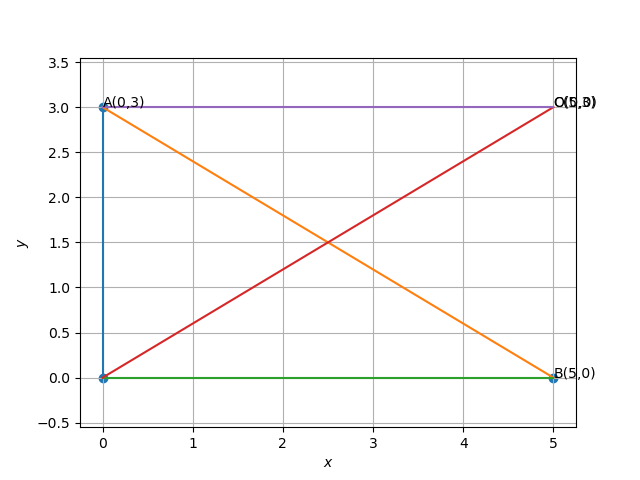
\includegraphics[width = 0.7\columnwidth]{figs/img.png}
    \caption*{}
    \label{figs}
\end{figure}

\end{document}
